\begin{homeworkProblem}
    \begin{enumerate}
        \item In Section 1.3 it was shown that the general solution to equation
        (16a, b) is (22) provided $\lambda_1 \neq \lambda_2$. Show that if
        $\lambda_1 = \lambda_2 = \lambda$ then the general solution is
        \[
            A_1\lambda^n + A_2 n \lambda^n.
        \]
        \item Solve and graph the solutions to each of the following equations or
        systems
        \begin{enumerate}[label=(\roman*)]
            \addtocounter{enumii}{1}
            \item $x_{n+2} - 2x_{n+1} + x_n = 0,$
            \item $x_{n+1} = -3 x_n - 2y_n,$\\
            $\qquad y_{n+1} = \phantom{-} 2 x_n +\phantom{2}y_n.$
        \end{enumerate}
    \end{enumerate}
    
    \segline
    
    \solution
    \begin{enumerate}
        % Solution 3(a)
        \item \textit{Proof} by Mathematical Induction:
        We know from (16a, b) that
        \[
            x_{n+2} = B_1 x_{n+1} + B_2 x_{n}
        \]
        is true for all $n$, where $B_1$ and $B_2$ are some constants.
        Suppose that $\lambda_0$ is the repeated solution to the characteristic
        equation
        \[
            \lambda^2 - B_1 \lambda - B_2 = 0
        \]
        By Vieta's formulas, we know that $B_1 = 2\lambda_0$ and $B_2=-\lambda_0^2$.
    
        Suppose that the general solution formula is true for all integers from $0$
        through $k$, then we have\[
        \begin{aligned}
            x_k &= A_1 \lambda_0^k + A_2 k \lambda_0^k,\\
            x_{k-1} &= A_1 \lambda_0^{k-1} + A_2 (k-1) \lambda_0^{k-1}.
        \end{aligned}
        \]
        For $x_{k+1}$, we have \[
            \begin{aligned}
                x_{k+1} &= B_1 x_{k} + B_2 x_{k-1}\\
                &= B_1 (A_1 \lambda^k + A_2 k \lambda^k) +
                B_2 (A_1 \lambda^{k-1} + A_2 (k-1) \lambda^{k-1})\\
                &= A_1 (B_1 \lambda^k + B_2 \lambda^{k-1}) +
                A_2 (B_1 k \lambda^k + B_2 (k-1) \lambda^{k-1})\\
                &= A_1 (2\lambda^{k+1} - \lambda^{k+1}) +
                A_2 (2k\lambda^{k+1} + (1-k) \lambda^{k+1})\\
                &= A_1 \lambda^{k+1} + A_2 (k+1) \lambda^{k+1}
            \end{aligned}
        \]
        The truth of $x_0$ and $x_1$ is automatic since $A_1$ and $A_2$ are numbers
        selected intentionally to make the following equations true: \[
            x_0 = A_1, \quad x_1 = (A_1 + A_2) \lambda.
        \]
        \begin{flushright}
            $\qed$
        \end{flushright}
    
        \pagebreak
        % Solution 3(b)
        \item Note: the constants $A_1$ and $A_2$ are se as $1$ for both questions.
        \begin{enumerate}[label=(\roman*)]
        \addtocounter{enumii}{1}
        % Solution 3(b)(ii)
            \item The characteristic equation is \[
                \lambda^2 - 2\lambda + 1 = 0.
            \]
            So the roots should be $\lambda_1 = \lambda_2 = \lambda = 1$.
            The general solution would be \[
                x_n = A_1 + A_2 n,
            \] since the power of $1$ is always $1$.
            \begin{figure}[H]
                \centering
                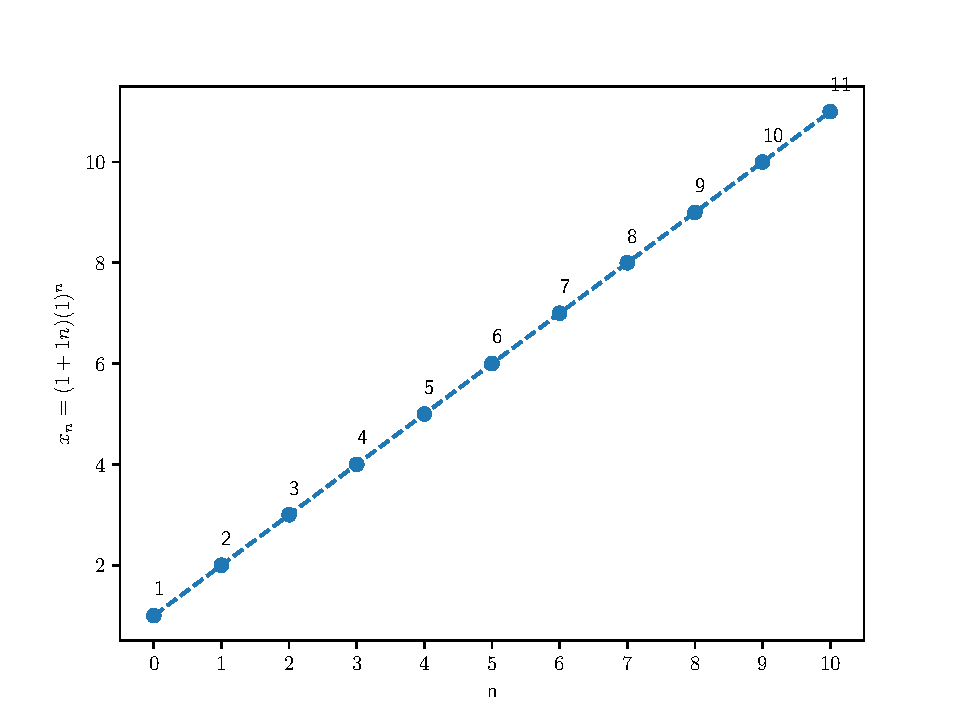
\includegraphics[scale=0.5]{fig/fig3(b)(ii).pdf}
            \end{figure}
    
        % Solution 3(b)(iii)
            \item The system of linear difference equation can be written in matrix form: \[
                \left(\begin{matrix}A_1\lambda^{n+1}\\ A_2\lambda^{n+1}\end{matrix}\right)
                = \left(\begin{matrix}
                    -3 & -2 \\
                     2 &  1
                \end{matrix}\right)
                \left(\begin{matrix}A_1\lambda^n \\ A_2 \lambda^n \end{matrix}\right)
            \qquad \Leftrightarrow \qquad
                \left(\begin{matrix}
                    -3-\lambda & -2 \\
                     2 &  1-\lambda
                \end{matrix}\right) \left(\begin{matrix}A\\B\end{matrix}\right)
                = 0
            \]
            Let determinant of the matrix of coefficients euqal to $0$, it leads to \[
                \mathbf{det}\left(\begin{matrix}
                    -3-\lambda & -2 \\
                     2 &  1-\lambda
                \end{matrix}\right) = 0 \qquad \Rightarrow \qquad
                \lambda^2 + 2\lambda + 1 = 0
            \]
            So we hanve two repeated eigenvalues $\lambda_1 = \lambda_2 = \lambda = -1$. And the
            general solution would be \[
                x_n = (A_1 + A_2 n) (-1)^n,
            \]
            \begin{figure}[H]
                \centering
                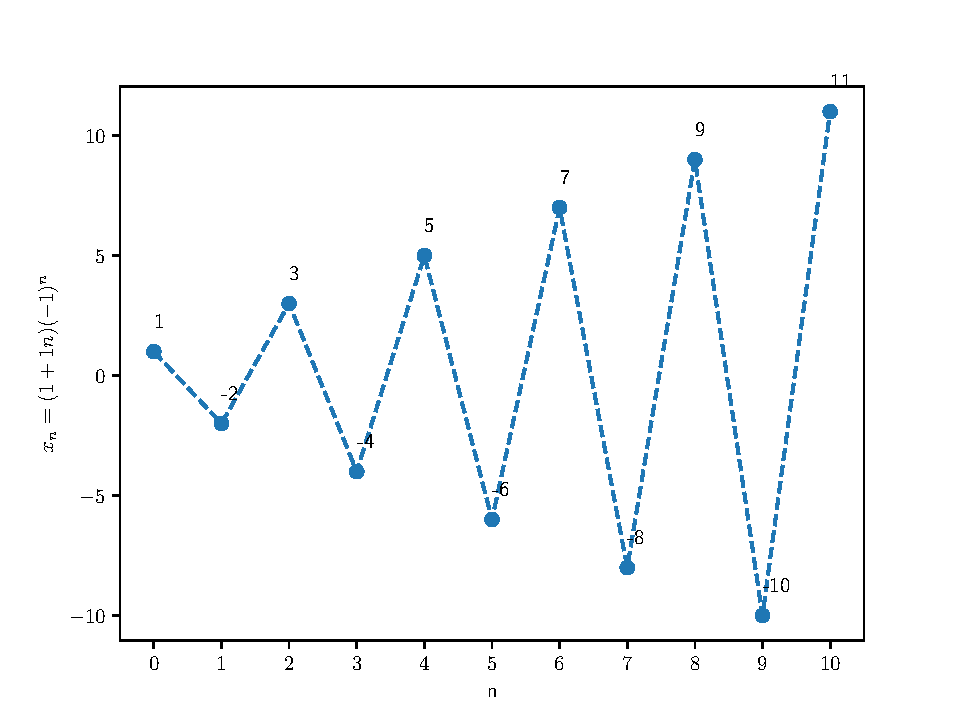
\includegraphics[scale=0.5]{fig/fig3(b)(iii).pdf}
            \end{figure}
        \end{enumerate}
    \end{enumerate}
    \end{homeworkProblem}